\section{Controlled Numerical Studies}
\label{sec:studies}

\subsection{What this evidence is, and what it cannot support}
\label{sec:studies-scope}

Everything in this section is a measurement of the \emph{mechanism}, taken against the reference implementation on constructed inputs whose ground truth we control. None of it is a language-modelling result, and none of it can substitute for one.

The reason to run these studies before training anything is that they are exact, cheap, and capable of falsifying claims. A perplexity number cannot tell you whether the router's partition collapsed, whether the load imbalance came from the router or the encoder, or whether the fast kernel computes the function the method describes; it aggregates all of those into one scalar that is also sensitive to a dozen unrelated choices. The studies below separate them. Two of them returned answers that contradicted what this paper previously asserted, which is the main argument for doing them in this order.

What they cannot show: whether any of this helps a trained model. In particular, every study here uses an \emph{untrained} router, so they measure the geometry the architecture imposes rather than what optimisation could make of it. Section~\ref{sec:s5} is the sharpest illustration --- it finds no difference between ablation arms at initialisation at all, which is itself a constraint on how the remaining claims can be tested.

\paragraph{Reproduction.} Each study writes a CSV; the tables and figures in this section are generated from those CSVs by a script, so no number here is transcribed by hand and the evidence regenerates end to end:

\begin{center}
\small\ttfamily
python experiments/numerical\_studies.py \&\& python experiments/make\_tables.py
\end{center}

\noindent Unless stated otherwise: $\dc$ and the bucket count $B = 2\dc$ as given per row; RoPE base $10^4$; Cayley-parametrised rotations at default initialisation; results averaged over 32 content directions for the routing studies and 4--8 random initialisations elsewhere; CPU, float32, seeds fixed and recorded.

\begin{figure}[t]
\centering
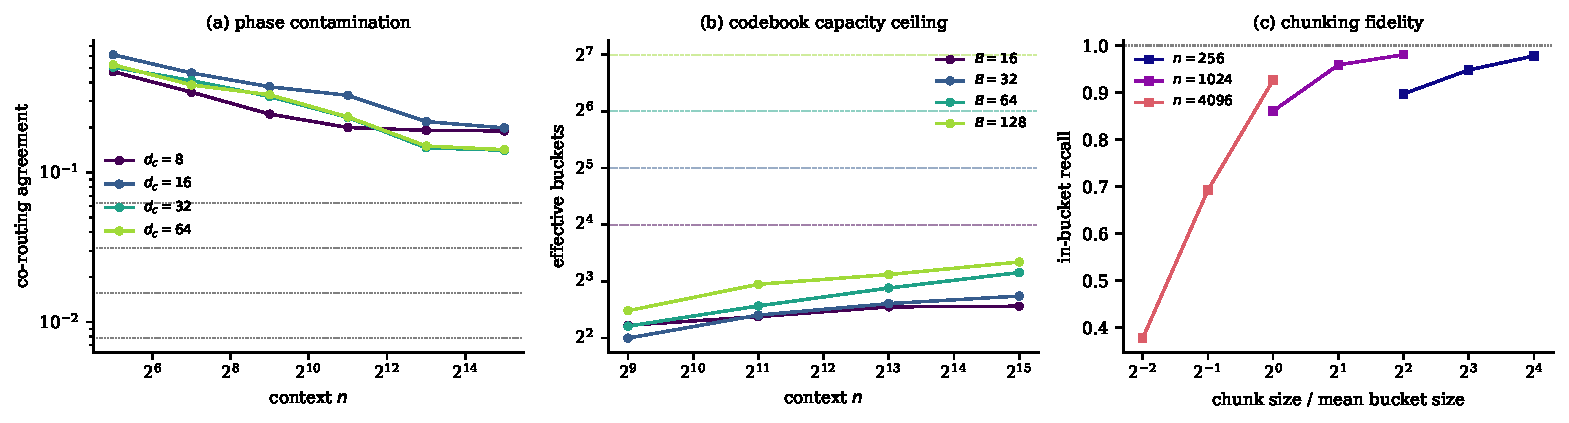
\includegraphics[width=\textwidth]{generated/studies.pdf}
\caption{The three findings that changed the paper. \textbf{(a)} Co-routing agreement for \emph{content-identical} tokens whose only difference is position, under RoPE-read routing, against context length. Dotted lines mark chance $1/B$ for each width. Agreement falls monotonically, as Proposition~\ref{prop:rope} predicts, but plateaus an order of magnitude above chance. \textbf{(b)} The reason: the number of \emph{effective} buckets the router reaches saturates near $6$--$10$ (dashed lines mark the provisioned $B$). Provisioning more buckets does not raise the ceiling, so the relative collapse worsens with $B$. \textbf{(c)} Fidelity of bucket-sorted fixed-size chunking to true bucket-wise attention, against the ratio of chunk size to mean bucket size. The three context lengths collapse onto one curve, identifying $c/\bar{m}$ as the governing variable; fidelity is lost below $c \approx \bar{m}$.}
\label{fig:studies}
\end{figure}

\subsection{S1 and S2: phase contamination and the capacity ceiling}
\label{sec:s1}
\label{sec:s2}

\paragraph{Construction.} A content vector $\bu$ is drawn and held fixed. It is placed at every position $0,\dots,n-1$, RoPE is applied, and the router is read. Any loss of co-routing is attributable to rotary phase and to nothing else, because the content never varies. We report the fraction of positions whose bucket matches position $0$ (``co-routing agreement''), and the perplexity of the visited-bucket distribution (``effective buckets''), averaged over 32 content directions.

\begin{table}[h]
\centering
\small
\begin{tabular}{llrrrrrrrr}
\toprule
 & & \multicolumn{4}{c}{co-routing agreement} & \multicolumn{4}{c}{effective buckets} \\
\cmidrule(lr){3-6}\cmidrule(lr){7-10}
$\dc$ & $B$ & \multicolumn{1}{c}{512} & \multicolumn{1}{c}{2048} & \multicolumn{1}{c}{8192} & \multicolumn{1}{c}{32768} & \multicolumn{1}{c}{512} & \multicolumn{1}{c}{2048} & \multicolumn{1}{c}{8192} & \multicolumn{1}{c}{32768} \\
\midrule
8 & 16 & 0.2462 & 0.2003 & 0.1917 & 0.1901 & 4.68 & 5.2 & 5.86 & 5.91 \\
16 & 32 & 0.375 & 0.3287 & 0.2193 & 0.1991 & 4.0 & 5.3 & 6.1 & 6.69 \\
32 & 64 & 0.3229 & 0.2341 & 0.1465 & 0.1411 & 4.63 & 5.93 & 7.38 & 8.92 \\
64 & 128 & 0.3314 & 0.2356 & 0.1506 & 0.1424 & 5.59 & 7.73 & 8.7 & 10.15 \\
\bottomrule
\end{tabular}
\caption{Phase contamination (S1) and codebook capacity (S2), by routing width and context length. Chance agreement is $1/B$: $0.063$, $0.031$, $0.016$, $0.008$ for the four widths. Agreement plateaus at roughly $0.14$--$0.20$ for every width, so its \emph{ratio} to chance grows from $3\times$ at $B=16$ to $18\times$ at $B=128$. The effective bucket count explains this: it saturates near $6$--$10$ regardless of $B$.}
\label{tab:s1s2}
\end{table}

\paragraph{What we had claimed.} Proposition~\ref{prop:rope} shows that for a \emph{single} rotary plane the co-routing probability tends to $1/B_2$ under equidistribution. We extrapolated from that to the whole head and wrote that content routing ``degenerates into position hashing''.

\paragraph{What the measurement shows.} The monotone decay is there and is robust: agreement falls from $0.61$ to $0.20$ at $\dc=16$, and the fall continues across four orders of magnitude of context. But it plateaus, and the plateau sits at $3$ to $18$ times chance depending on width. The effective bucket count in the right half of Table~\ref{tab:s1s2} identifies the cause: the router never reaches more than about ten buckets, however many exist. At $B=16$ that is $37\%$ of the codebook; at $B=128$ it is $8\%$.

\begin{revision}{Correction to the paper's claim}
Routing on rotary dimensions does not degrade toward uniform hashing. It degrades toward a \textbf{capacity ceiling}: a small, nearly width-independent number of reachable buckets. This is a worse failure than uniform hashing, not a milder one --- the model loses content selectivity \emph{and} most of its bucket capacity, and the loss of capacity gets relatively worse the more capacity is provisioned. Proposition~\ref{prop:rope} stands as stated, per plane. Its extrapolation to the head does not, and we have replaced it.
\end{revision}

\paragraph{Why.} The mechanism is geometric and exact.

\begin{proposition}[Torus confinement]
\label{prop:torus}
Let $\hat\bu \in S^{\dc - 1}$ be a fixed unit content vector with $\dc = 2h$, and let $\bw(m) = \Theta_m \hat\bu$ be its RoPE image at position $m$, where $\Theta_m$ is block-diagonal with $h$ planar rotations of angles $\theta_1 m, \dots, \theta_h m$. Then for all $m$,
\begin{equation}
  \bw(m) \in \mathcal{T}(\hat\bu) \;=\; \Big\{ \bx \in \R^{\dc} : \|(x_j, x_{j+h})\| = E_j(\hat\bu) \;\; \forall j \le h \Big\},
\end{equation}
an $h$-dimensional torus embedded in $S^{\dc-1}$, where $E_j$ is the fixed energy of plane $j$. Consequently the set of routing inputs reachable by varying position alone has measure zero in $S^{\dc-1}$, and the set of buckets reachable by $\hat\bu$ is bounded by the number of cells of the partition that $\bR\,\mathcal{T}(\hat\bu)$ meets --- a quantity governed by $h = \dc/2$, not by $B$.
\end{proposition}

\begin{proof}
Each $2\times2$ block of $\Theta_m$ is a rotation and therefore preserves the norm of the corresponding coordinate pair, so $E_j$ is constant in $m$. The set of points with all $h$ plane norms fixed is a product of $h$ circles. Its dimension is $h = \dc/2 < \dc - 1$ for $\dc > 2$, hence measure zero in the sphere. The reachable bucket set is the image of this torus under the orthogonal $\bR$, intersected with the $B$ cells of the cross-polytope partition; an $h$-dimensional set meets a number of cells that grows with $h$, and $\bR$ being orthogonal does not change the dimension.
\end{proof}

This predicts slow growth of the ceiling with $\dc$ and no dependence on $B$ beyond the $B = 2\dc$ coupling, which is what Table~\ref{tab:s1s2} shows: quadrupling $h$ from 4 to 32 moves the effective bucket count only from $5.9$ to $10.2$. It also explains why the plateau value of agreement is roughly width-independent while its ratio to chance is not.

\paragraph{Consequence for the protocol.} The diagnostic E0 must report \emph{effective bucket count}, not only mutual information between bucket and position. We also found that mutual information with binned position is non-monotone in context length --- it peaks when the phase has advanced enough to correlate with position but not enough to scramble it --- and is therefore a misleading headline metric. The quantity that falls monotonically is the mutual information between cluster and \emph{token identity}. Section~\ref{sec:protocol} reflects both corrections.

\subsection{S3: the load belongs to the data, not to the router}
\label{sec:s3}

\paragraph{Construction.} Routing inputs are drawn as $\bu \sim \mathcal{N}(\kappa \be_1, \bI)$ for a concentration parameter $\kappa$ interpolating from isotropic ($\kappa = 0$) to strongly anisotropic. For each, we record the normalised load entropy at initialisation, and again after 300 Adam steps on an objective that explicitly rewards pushing every token into bucket $0$ --- the most direct collapse pressure available to the router.

\begin{table}[h]
\centering
\small
\begin{tabular}{lrrrr}
\toprule
$\kappa$ & $H(\pi)/\log B$ at init & after pressure & $\Delta$ & buckets used \\
\midrule
0.0 & 0.9994 & 0.9994 & -0.0 & 32 \\
0.25 & 0.9968 & 0.9967 & -0.0001 & 32 \\
0.5 & 0.9877 & 0.9884 & 0.0007 & 32 \\
1.0 & 0.9473 & 0.9476 & 0.0003 & 32 \\
2.0 & 0.7151 & 0.7059 & -0.0092 & 32 \\
4.0 & 0.1024 & 0.0787 & -0.0237 & 31 \\
\bottomrule
\end{tabular}
\caption{Load entropy against input anisotropy $\kappa$, before and after 300 steps of explicit collapse pressure on the rotation ($\dc=16$, $B=32$, $n=8192$). The load is determined almost entirely by $\kappa$; the pressure moves it by at most $0.024$.}
\label{tab:s3}
\end{table}

\paragraph{What the measurement shows.} Load entropy is a clean monotone function of input concentration, falling from $0.999$ at $\kappa=0$ to $0.102$ at $\kappa=4$. The effect of 300 steps of adversarial optimisation on the router is at most $0.024$ and is usually within noise of zero. At the isotropic end it is exactly zero to four decimals. This is not an artefact of the optimiser; it is forced:

\begin{proposition}[Load is a property of the data]
\label{prop:load}
Let the routing input $\bu$ be drawn from a rotationally invariant distribution on $\R^{\dc}$. Then under Definition~\ref{def:router} the bucket marginal $\pi$ is uniform for \emph{every} $\bR \in O(\dc)$, and is therefore invariant to the router's parameters.
\end{proposition}
\begin{proof}
If $\bu$ is isotropic then so is $\bR\hat\bu$ for orthogonal $\bR$, since orthogonal maps preserve rotational invariance. The cross-polytope sectors are congruent under the symmetry group of the codebook, so an isotropic direction falls in each with equal probability.
\end{proof}

\begin{revision}{This invalidated one of our own ablations}
Ablation A6 was specified as a sweep over the coefficient $\lambda$ of a balancing loss placed on the router, to test whether orthogonality reduces the balancing needed. Proposition~\ref{prop:load} says the experiment cannot work: a loss whose gradient reaches only $\bR$ cannot change a marginal that does not depend on $\bR$. Balancing has to act on the \emph{encoder} that produces the routing input, or the input must be whitened before the router sees it. A6 is respecified in Section~\ref{sec:protocol} with a whitening arm, and we flag that the original design would have produced a null result that we might have misread as evidence for the method.
\end{revision}

Two further consequences. First, Section~\ref{sec:limits}'s ``load collapse survives'' is now a sharper and more testable claim: load collapse is attributable \emph{entirely} to anisotropy of the encoder's output. Second, Proposition~\ref{prop:load} is a genuine guarantee in the isotropic regime and comes for free with the orthogonality constraint, which no unconstrained router can offer.

\subsection{S4: the codebook geometry is rigid, and a free router's is not}
\label{sec:s4}

\paragraph{Construction.} Proposition~\ref{prop:collapse} is a statement about reachability: the minimum prototype angle of an unconstrained router \emph{can} be driven to zero by gradient descent, and ours cannot, for any parameter value. The honest test is therefore adversarial rather than task-shaped --- we optimise directly against the quantity in both families, maximising mean pairwise prototype cosine similarity, and watch the minimum angle.

\begin{table}[h]
\centering
\small
\begin{tabular}{lrrrr}
\toprule
router & step 0 & step 50 & step 150 & step 400 \\
\midrule
orthogonal (ours) & 90.0 & 90.0 & 90.0 & 90.0 \\
unconstrained linear & 48.43 & 0.809 & 0.0 & 0.0 \\
\bottomrule
\end{tabular}
\caption{Minimum angle between distinct, non-antipodal bucket prototypes (degrees) under an objective that explicitly rewards collapse ($\dc=16$, $B=32$). The orthogonal router is unmoved at every step; the unconstrained router collapses completely within 150 steps.}
\label{tab:s4}
\end{table}

\paragraph{What the measurement shows.} Exactly what Proposition~\ref{prop:collapse} asserts, with no slack: the orthogonal router's minimum prototype angle is $90.000^\circ$ at step 0 and $90.000^\circ$ at step 400, while the unconstrained router goes from $48.4^\circ$ to $0.8^\circ$ in 50 steps and to $0.0^\circ$ by 150. The orthogonality is exact rather than penalty-enforced, so this is a structural property and not a tuning outcome.

\paragraph{What it does not show.} That this matters for language modelling. Representation collapse as documented by \citet{chi2022representation} is an empirical pathology of trained MoE systems, and we have demonstrated only that one channel for it is closed by construction. Proposition~\ref{prop:load} and S3 show that the other channel --- data-side concentration --- remains fully open, and is the one more likely to bite.

\subsection{S5: at initialisation, the ablation arms are indistinguishable}
\label{sec:s5}

\paragraph{Construction.} For each ablation arm we measure the fraction of \emph{dense} top-$k$ attention mass that the sparse pattern retains (``recall''), against the fraction of causal cells the pattern admits (``density''). A random pattern of equal density has expected recall equal to its density, so the ratio is the pattern's selectivity. We run two input regimes: Gaussian noise, and sequences drawn from 32 recurring token embeddings --- the latter because real text repeats token types across distant positions, which is the structure a content router is supposed to exploit.

\begin{table}[h]
\centering
\small
\begin{tabular}{llrrrr}
\toprule
input & variant & $n$ & density & top-$k$ recall & recall/density \\
\midrule
gaussian & phasor & 256 & 0.0909 & 0.2735 & 3.008 \\
gaussian & phasor & 1024 & 0.0464 & 0.2105 & 4.54 \\
gaussian & a1\_frozen\_rotation & 256 & 0.0907 & 0.2736 & 3.015 \\
gaussian & a1\_frozen\_rotation & 1024 & 0.0464 & 0.211 & 4.549 \\
gaussian & a3\_route\_on\_rope & 256 & 0.0908 & 0.2738 & 3.015 \\
gaussian & a3\_route\_on\_rope & 1024 & 0.0463 & 0.2107 & 4.547 \\
gaussian & a4\_pure\_skip & 256 & 0.0909 & 0.2735 & 3.008 \\
gaussian & a4\_pure\_skip & 1024 & 0.0464 & 0.2105 & 4.54 \\
structured & phasor & 256 & 0.0892 & 0.2691 & 3.017 \\
structured & phasor & 1024 & 0.0456 & 0.206 & 4.517 \\
structured & a1\_frozen\_rotation & 256 & 0.0911 & 0.2719 & 2.985 \\
structured & a1\_frozen\_rotation & 1024 & 0.0467 & 0.2086 & 4.469 \\
structured & a3\_route\_on\_rope & 256 & 0.091 & 0.2743 & 3.013 \\
structured & a3\_route\_on\_rope & 1024 & 0.0462 & 0.2158 & 4.672 \\
structured & a4\_pure\_skip & 256 & 0.0892 & 0.2691 & 3.017 \\
structured & a4\_pure\_skip & 1024 & 0.0456 & 0.206 & 4.517 \\
\bottomrule
\end{tabular}
\caption{Pattern selectivity at initialisation ($d=128$, 4 heads, window 8, $k=32$). Angular bucketing beats a random pattern of equal density by a factor of three to five, but no arm is distinguishable from any other, in either input regime.}
\label{tab:s5}
\end{table}

\paragraph{What the measurement shows.} Two things, and the second is the useful one.

The cross-polytope partition is a genuinely good pattern prior: recall exceeds density by $2.5$ to $4.7$ times, and the margin \emph{grows} with context ($3.0\times$ at $n=256$, $4.5\times$ at $n=1024$ for the same window). Angular bucketing is doing real work relative to selecting the same number of keys at random.

But every arm does it equally well. Learned rotation, frozen random rotation, routing on content dimensions, routing on rotary dimensions, with and without residue summaries --- all land within $0.011$ of each other in recall at matched density, under both input regimes. Planting content structure in the input does not separate them either.

\begin{revision}{Constraint on how A1 and A3 can be tested}
Pattern geometry at initialisation carries no information about which routing rule is better. Any difference between the ablation arms must be \emph{created by training}, which means A1 (learned versus frozen rotation) and A3 (content versus rotary routing) cannot be settled by cheap pattern-quality measurement and require full training runs. It also means a reader should treat an initialisation-time pattern comparison --- ours or anyone's --- as uninformative about routing rules.
\end{revision}

This is the clearest reason the fixed-hash null of \citet{roller2021hash} has to be taken seriously: before training, our learned router and Reformer's random one are the same pattern.

\subsection{S6: the residue branch is a free hyperparameter the paper did not declare}
\label{sec:s6}

\begin{table}[h]
\centering
\small
\begin{tabular}{lrl}
\toprule
bias at init & residue mass & inside P3's 2--25\% band \\
\midrule
0.0 & 0.6178 & no \\
-2.0 & 0.1881 & yes \\
-4.0 & 0.031 & yes \\
-6.0 & 0.0043 & no \\
-8.0 & 0.0006 & no \\
\bottomrule
\end{tabular}
\caption{Fraction of attention mass taken by the residue branch at initialisation, against its logit bias ($d=128$, 4 heads, $n=512$, window 8). Prediction P3 assumes a $2$--$25\%$ band; only two of the five settings reach it, and the default of zero is far outside.}
\label{tab:s6}
\end{table}

With the residue logits entering the shared softmax at zero bias, the branch takes $62\%$ of the attention mass before any training. Prediction P3 states that mass near one would indicate ``routing has failed''; at initialisation it indicates nothing except that $B$ well-conditioned logits compete against a sparse fine branch. The implementation now initialises the bias to $-4$, which starts the branch at $3\%$.

Two consequences. P3 must be a statement about the \emph{converged} model and the paper must declare the initialisation, or the prediction is unfalsifiable because its outcome is settable. And the initialisation is a hyperparameter nobody has tuned, plausibly as consequential as anything else in ablation A4; it is now swept there.

\subsection{S7: chunking is faithful only when the chunk matches the bucket}
\label{sec:s7}

\paragraph{Construction.} The $O(n^{1.5})$ complexity in Section~\ref{sec:complexity} depends on sorting tokens by bucket and attending within fixed-size chunks, as Reformer does. That is not the same function as attending within buckets: a bucket larger than the chunk is split and loses intra-bucket pairs, and a smaller one is padded with a neighbouring bucket's tokens. We measure the gap on the \emph{pattern}, which requires no fast kernel. We report in-bucket recall (the fraction of true causal in-bucket pairs the chunked pattern keeps) and contamination (the fraction of the chunked pattern's pairs that are not in-bucket at all).

\begin{table}[h]
\centering
\small
\begin{tabular}{rrrrrr}
\toprule
$n$ & chunk $c$ & $c / \bar{m}$ & $H(\pi)/\log B$ & in-bucket recall & contamination \\
\midrule
256 & 32 & 4.00 & 0.978 & 0.8972 & 0.8811 \\
256 & 64 & 8.00 & 0.978 & 0.948 & 0.9328 \\
256 & 128 & 16.00 & 0.978 & 0.9777 & 0.9594 \\
1024 & 32 & 1.00 & 0.992 & 0.8607 & 0.5634 \\
1024 & 64 & 2.00 & 0.992 & 0.9588 & 0.7532 \\
1024 & 128 & 4.00 & 0.992 & 0.9803 & 0.8699 \\
4096 & 32 & 0.25 & 0.996 & 0.3779 & 0.2632 \\
4096 & 64 & 0.50 & 0.996 & 0.6927 & 0.3074 \\
4096 & 128 & 1.00 & 0.996 & 0.9265 & 0.5313 \\
\bottomrule
\end{tabular}
\caption{Fidelity of bucket-sorted fixed-size chunking ($d=128$, 4 heads, $B=32$, window 1). $\bar{m} = n/B$ is the mean bucket size. Load entropy is near-perfect throughout, so the loss of fidelity is not an imbalance artefact.}
\label{tab:s7}
\end{table}

\paragraph{What the measurement shows.} At $n=4096$ with chunk $32$, the chunked pattern retains $38\%$ of true in-bucket pairs. Load entropy in the same runs is $0.996$, so this is not caused by unbalanced buckets --- it is intrinsic. Figure~\ref{fig:studies}(c) identifies the governing variable: plotted against $c/\bar{m}$, the three context lengths collapse onto a single curve. Fidelity above $90\%$ requires $c \gtrsim \bar{m} = n/B$.

\paragraph{What this does to the complexity claim.} Section~\ref{sec:complexity} balanced the in-bucket term $n^2/B$ against the residue term $nB$ and obtained $B \asymp \sqrt{n}$, hence $O(n^{1.5})$. The chunk-fidelity requirement adds a constraint the analysis omitted: $c \gtrsim n/B$, so the in-bucket work per query is $\Omega(n/B)$ and the total is $\Omega(n^2/B)$ --- which is $O(n^{1.5})$ only if $B$ grows as $\sqrt{n}$. Under Definition~\ref{def:router}, $B = 2\dc$ is the head's content width. So reaching the claimed operating point at context $n$ requires
\begin{equation}
  \dc \;\approx\; \tfrac{1}{2}\sqrt{n},
\end{equation}
that is, $\dc = 32$ at $n = 4096$ and $\dc = 128$ at $n = 65{,}536$. The first is ordinary; the second is a $128$-dimensional content subspace per head on top of the positional dimensions, which is a real architectural cost that the complexity figure hides.

\begin{revision}{Qualification of the complexity claim}
The $O(n^{1.5})$ figure is not wrong, but it is conditional on an operating point the paper did not state: the routing width must scale as $\sqrt{n}$, because $B = 2\dc$ and chunk fidelity requires $c \gtrsim n/B$. At fixed $\dc$ the method is quadratic with constant $1/B$. Multi-round routing relaxes the constraint by unioning $n_r$ independent partitions, at cost linear in $n_r$; whether that is a better trade than widening $\dc$ is an open question we have not measured. Any wall-clock claim must report in-bucket recall alongside it, or it is reporting the speed of a different function from the one the method defines.
\end{revision}

\subsection{Toy-scale ablations, and a trap in how they are budgeted}
\label{sec:toy}

The reference implementation applies routing as a mask over the full $(n,n)$ score matrix, so it is $O(n^2)$ and says nothing about speed; what it can do is check that an arm trains. We run the arms on a synthetic copying task --- the second half of each sequence repeats the first half --- which is sensitive to exactly the long-range dependency sparse attention can break, unlike random tokens, where every pattern scores the same. \textbf{The sweep is incomplete at the time of writing}; Table~\ref{tab:ablation} lists the arms that have finished.

\begin{table}[h]
\centering
\small
\begin{tabular}{lrrrr}
\toprule
arm & params & best loss (seed 0 / 1) & density & $H(\pi)/\log B$ \\
\midrule
dense & 393\,856 & 3.870 / 3.434 & 1.000 & -- \\
phasor & 394\,384 & 4.160 / 4.158 & 0.086 & 0.738 \\
\bottomrule
\end{tabular}
\caption{Toy scale, \textbf{sweep incomplete}: 2 layers, $d = 128$, 4 heads, context 256, vocabulary 64, 1000 steps, two seeds reported separately. These runs cannot support a claim about language modelling. The unigram floor is $\log 64 = 4.159$; PHASOR's density is $8.6\%$ at window 8.}
\label{tab:ablation}
\end{table}

\paragraph{What the numbers say, read naively.} Dense reaches $3.43$ and $3.87$; PHASOR sits at $4.160$ and $4.158$ --- the unigram floor to three decimals, on both seeds. Read as a result, this says the sparse arm cannot do the task.

\paragraph{What the trajectories say.} They do not support that reading. The loss curves are flat at the floor and then fall sharply: dense seed 1 leaves the floor at step 400 and reaches $3.43$; dense seed 0 stays at the floor until step 900 and has only reached $3.87$ when the budget ends. The task is learned by a phase transition whose \emph{onset time} varies by more than a factor of two across seeds of an otherwise identical configuration. PHASOR's two seeds are both still flat at step 1000.

So the honest statement is narrow: within a budget in which the dense baseline barely completes its transition, PHASOR has not begun one. Whether it would at step 2000 or 5000 is unmeasured, and nothing here licenses the claim that it cannot.

\begin{revision}{A trap in budgeting sparse-attention comparisons}
If the training budget is set so that the dense baseline is near its phase transition rather than well past it, every slower-onset arm reports at the floor and the comparison appears decisive when it is only truncated. Our own first reading of this table fell into it. Any budget for A1/A3/A4 must be long enough that \emph{the dense arm has plateaued}, not merely long enough that it has started to learn --- and the trajectories, not the final numbers, must be reported so a reader can tell the difference.
\end{revision}

Taken with S5 --- the arms are indistinguishable before training --- the position is that A1 and A3 require training runs that are both long enough to pass the transition and replicated enough to resolve onset-time variance. Section~\ref{sec:protocol} specifies that. Nothing cheaper will do, which is the single most expensive consequence of this report's findings.
